\documentclass[11pt, a4paper, jou]{apa7}
\setlength{\headheight}{14pt}
\usepackage[style=numeric]{biblatex}

\usepackage{hyperref}
\usepackage{url}
\usepackage{graphicx}
\usepackage{epstopdf}
\usepackage{longtable}

\addbibresource{Ref.bib}

\leftheader{ZEHAO WANG}

\linespread{1.5}
\title{Will it rain tomorrow? --- Course Report on Weather Prediction}
\shorttitle{BIOS-7650 COURSE PROJECT}
\author{Zehao Wang}
\authorsaffiliations{Master student in Statistics, Department of Mathematics}
\course{BIOS-7650 Statistical Learning in Data Science}
\professor{Dr.\ Li. }
\duedate{\today}
\abstract{
    In this report, we use the weather dataset from \href{https://www.kaggle.com/datasets/jsphyg/weather-dataset-rattle-package}{Kaggle} to predict the weather. We first modeled the data with logistic regression, achieving an accuracy of about $85.045\%$ on the test set. Then the SVM with kernel trick was used, achieving $90\%$ accuracy on the same test set. Finally, we used the current mainstream method of machine learning, neural networks, to achieve an accuracy of $95\%$. And the code can be found in \href{\url{https://github.com/Addasecond86/MS-Stat-Tulane/tree/main/Stat%20Learning%20in%20Data%20Analysis/Project/Code}}{Kaggle}. 
}
\begin{document}
\maketitle
\section{Methods}
Before we start fitting the data, we first need to clean it. For missing value, I dropped the subjects that had missing values in the variables \emph{RainToday} and \emph{RainTomorrow}. Because I have no good idea to fill in the missing values in these two variables. For other continuous variables, it is not appropriate to fill the missing values with $0$, because variables such as temperature and barometric pressure cannot be $0$ even if they are missing. So I use the median of the current month to substitute the missing values of these continuous variables. For the remaining categorical variables, the missing values are not so important, because they are coded as dummy variables in the model. 
\subsection{Logistic Regression}
    Logistic regression\cite{Berkson1944} is widely used in binary classification problems. Assume $p$ is the probability of rain tomorrow, then, for logistic regression, we have
    \begin{equation}
        \frac{p}{1-p}=\exp\left(\beta_0+\sum_{i=1}^{n}\beta_i x_i\right). 
    \end{equation}
    And we can estimate the coefficients $\beta_i$ by maximum likelihood estimation. 

    We first use all the variables except the date as predictor variables to predict whether it will rain tomorrow. Further, we use stepwise to explore whether the model can be further optimized. Akaike information criterion (AIC)\cite{Akaike1974} was used to see if any of the variables can be eliminated. AIC is a measure of the relative quality of statistical models for a given set of data. It is defined as
    \begin{equation}
        {AIC} \,=\,2k-2\ln({\hat {L}}). 
    \end{equation}
    And $k$ is the number of estimated parameters in the model, $\hat{L}$ is the maximized value of the likelihood function for the model. So, the preferred model is the one with the minimum AIC value. 
\subsection{SVM}
    Support Vector Machine (SVM) is a better method than logistic regression, it tries to maximize the margin between two different classes of data points. 

\section{Results}

\subsection{Logistic Regression}
    Use $80\%$ as training set and $20\%$ as test set, logistic regression model with all the variables except the date has an accuracy of $85.045\%$ on the test set. And the accuracy on train set is $85.015\%$. The Confusion matrix is shown in figure~\ref{fig:logistic_confusion}. The accuracy and recall of this model are shown in table~\ref{tab:logistic_summary}. It can be seen that the accuracy ($0.87$) and recall ($0.95$) of the model are quite high with \emph{RainTomorrow} as \emph{No}. But it doesn't do well on data with \emph{RainTomorrow} as \emph{Yes}. 

    Next, we start from the full model and use AIC as a criterion to see if any variables can be excluded. The full process of stepwise is shown in table~\ref{tab:model_selection_aic}. Unfortunately, the AIC value of the full model is the smallest, so we cannot exclude any variables. 

    
    


\section{Discussion}

    

\printbibliography 
\clearpage
\appendix
\section{Figures and Tables}
\begin{figure}[p]
    \centering
    \caption{Confusion matrix of logistic regression model}\label{fig:logistic_confusion}
    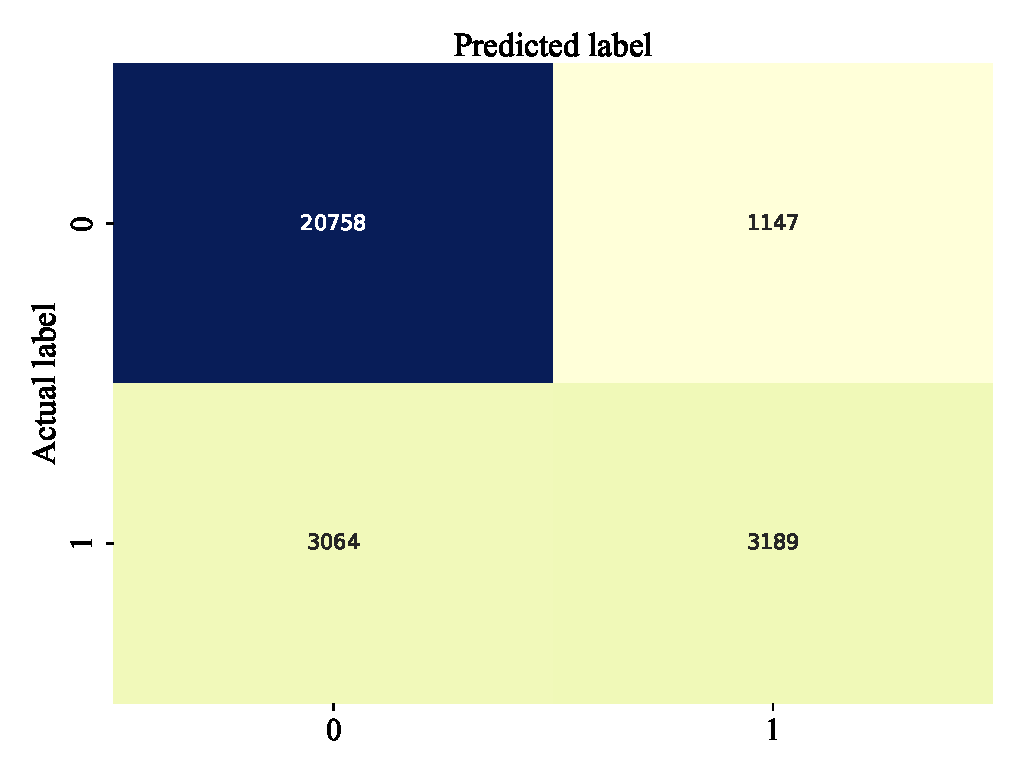
\includegraphics[width=.45\textwidth]{figures/Logit_confusion_matrix.eps}
\end{figure}

\begin{table}[p]
    \centering
    \caption{Logistic regression model summary}
    \label{tab:logistic_summary}
    \resizebox{\columnwidth}{!}{%
    \begin{tabular}{rrrrr}
    \hline
                 & precision & recall & f1-score & support \\ \hline
    Not Raining  & 0.87      & 0.95   & 0.91     & 21905   \\
    Raining      & 0.74      & 0.51   & 0.60     & 6253    \\
    accuracy     &           &        & 0.85     & 28158   \\
    macro avg    & 0.80      & 0.73   & 0.76     & 28158   \\
    weighted avg & 0.84      & 0.85   & 0.84     & 28158   \\ \hline
    \end{tabular}%
    }
\end{table}


\begin{table}[p]
    \centering
    \caption{Model selection for logistic regression with AIC as criterion}
    \label{tab:model_selection_aic}
    \begin{tabular}{lrrr}
    \hline
                   & Df & Deviance & AIC                          \\ \hline
    Full Model     &    & 84109    & {\color[HTML]{FE0000} 84327} \\
    -Temp3pm       & 1  & 84116    & 84332                        \\
    -Cloud9am      & 1  & 84116    & 84332                        \\
    -Evaporation   & 1  & 84118    & 84334                        \\
    -Humidity9am   & 1  & 84127    & 84343                        \\
    -WindGustDir   & 15 & 84156    & 84344                        \\
    -MinTemp       & 1  & 84136    & 84352                        \\
    -Temp9am       & 1  & 84143    & 84359                        \\
    -WindSpeed9am  & 1  & 84162    & 84378                        \\
    -Rainfall      & 1  & 84163    & 84379                        \\
    -MaxTemp       & 1  & 84201    & 84417                        \\
    -WindDir9am    & 15 & 84299    & 84487                        \\
    -WindDir3pm    & 15 & 84312    & 84500                        \\
    -WindSpeed3pm  & 1  & 84459    & 84675                        \\
    -RainToday     & 1  & 84479    & 84695                        \\
    -Sunshine      & 1  & 84552    & 84768                        \\
    -Cloud3pm      & 1  & 84788    & 85004                        \\
    -Pressure9am   & 1  & 84815    & 85031                        \\
    -Pressure3pm   & 1  & 85388    & 85604                        \\
    -Location      & 46 & 86546    & 86672                        \\
    -WindGustSpeed & 1  & 87564    & 87780                        \\
    -Humidity3pm   & 1  & 87902    & 88118                        \\ \hline
    \end{tabular}
    \end{table}
    

\begin{figure}[p]
    \centering
    \caption{ROC for logistic regression model}\label{fig:logistic_roc}
    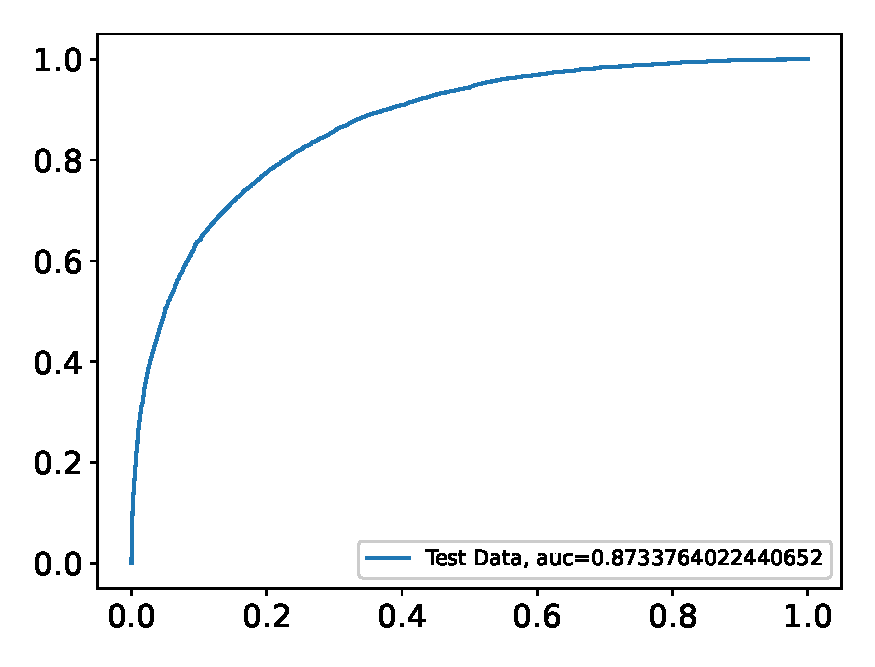
\includegraphics[width=.45\textwidth]{figures/Roc.eps}
\end{figure}
\end{document}